\documentclass[12pt]{article}
\usepackage{amsmath}
\usepackage{amssymb}
\usepackage{graphicx}
\usepackage{hyperref}
\usepackage{geometry}

\geometry{a4paper, margin=1in}


\hypersetup{
colorlinks=true,
linkcolor=blue,
filecolor=blue,      
urlcolor=blue,
}

\setlength{\parindent}{0pt}
\setlength{\parskip}{1em}

\title{Intro to AI \\ Assignment 2}
\author{Nikita Zagainov \\ DSAI-1}
\date{\today}

\begin{document}

\maketitle

\section{Implementation Details}
The algorithm for solving Sudoku is implemented in
\texttt{Python} and \texttt{C++} programming languages.
The \texttt{Python} implementation is used for experiments
and evaluation on test cases, while the \texttt{C++}
implementation is used as submission on CodeForces.

For better availability of implementation details,
I provide the source code on github:
\href{https://github.com/V1adych/itai-genetic-sudoku-solver}{Link}

\subsection{Individual}
As an individual for GA, I use matrices
of size $9 \times 9$ to represent a Sudoku
board with numbers from 1 to 9.
each individual has a constraint to
have specific numbers on specific
cells, which were given in the initial
sudoku board. This constrain is kept through the
whole evolution process.

\subsection{Fitness Function}
The fitness function is used to evaluate
individuals is the calculates the number of
distinct numbers in each row, column, and
$3 \times 3$ subgrid, then subtracts this number from 9
and sums all results up. The sudoku puzzle is solved
when the fitness function returns 0.

\subsection{Selection Process}
During one generation of the algorithm, all individuals
in population are evaluated on fitness function,
then the best individuals are selected for the next
generation and crossover process. Additionally,
stagnation is checked to prevent the algorithm from
running forever. If the best fitness is not improved
for a certain number of generations, the algorithm
resets the population entirely

\subsection{Crossover}
The crossover process is implemented as a simple
random selection of rows between two parents and
then combining them into a child.

\subsection{Mutation}
The mutation process is implemented as a random
switch of two numbers in a randomly chosen row.
Mutation happens with a certain probability with every
individual in the end of the generation.

\subsection{Hyperparameters}
The set of hyperparameters was chosen using
\href{https://arxiv.org/abs/1807.01774}{\texttt{BOHB}}
algorithm. The optimal set of hyperparameters:
\begin{itemize}
	\item Population size: 1400
	\item Max stagnation: 50
	\item Mutation chance: 0.95
	\item Elitism count: 700
\end{itemize}

This set of hyperparameters was used for evaluation on
\texttt{Python} implementation for tests. The final
implementation in \texttt{C++} used increased sizes of
population and elitism count to speed up the process.

\section{Test Cases}
We evaluated the genetic algorithm on various
Sudoku test cases with different numbers of
givens and complexity levels. The test cases
were divided into easy, medium, hard levels.
The definitions (approximate ranges of givens) 
of these levels were taken
from \href{https://www.sudoku.com}{sudoku.com}.

The following numbers of givens were used:
\begin{itemize}
	\item Easy: 42 givens
	\item Medium: 32 givens
	\item Hard: 28 givens
\end{itemize}

\section{Evaluation}
The evaluation was conducted on 30 different sudoku inputs
(all of which can be found in the \texttt{puzzles} folder
of \href{https://github.com/V1adych/itai-genetic-sudoku-solver}{GitHub repository}).

Some examples of them:
\subsection{Easy}
\begin{center}
	\begin{tabular}{|c|c|c|c|c|c|c|c|c|}
		\hline
		9 & 5 & 4 & 6 & 7 & 2 & 8 & - & 3 \\ \hline
		- & - & 8 & 1 & - & 9 & - & - & - \\ \hline
		- & - & - & - & - & 3 & 5 & 6 & - \\ \hline
		- & - & 5 & 3 & 4 & - & 6 & - & 7 \\ \hline
		- & - & 3 & 2 & 9 & 8 & 1 & - & - \\ \hline
		4 & - & 1 & 5 & 6 & - & - & 3 & - \\ \hline
		- & - & - & - & 3 & 6 & 2 & - & - \\ \hline
		- & 4 & 2 & 9 & - & - & - & 8 & - \\ \hline
		- & 3 & 6 & - & 2 & 4 & 7 & 9 & - \\ \hline
	\end{tabular}
\end{center}

\subsection{Medium}
\begin{center}
	\begin{tabular}{|c|c|c|c|c|c|c|c|c|}
		\hline
		- & - & - & - & 7 & - & - & 1 & 3 \\ \hline
		- & - & - & - & 5 & - & 4 & 7 & - \\ \hline
		- & 1 & 7 & - & 8 & 3 & 5 & - & 9 \\ \hline
		- & 9 & - & 3 & 4 & - & - & - & 7 \\ \hline
		6 & 7 & - & 2 & - & 8 & - & - & 5 \\ \hline
		- & - & - & 5 & 6 & 7 & - & 3 & - \\ \hline
		- & - & - & - & 3 & - & 2 & - & - \\ \hline
		7 & 4 & - & - & 1 & 5 & - & - & - \\ \hline
		- & - & - & - & - & - & 7 & - & - \\ \hline
	\end{tabular}
\end{center}

\subsection{Hard}
\begin{center}
	\begin{tabular}{|c|c|c|c|c|c|c|c|c|}
		\hline
		- & - & 4 & - & - & - & - & - & 3 \\ \hline
		- & - & 8 & - & - & - & - & - & 2 \\ \hline
		2 & - & - & - & - & - & - & - & 9 \\ \hline
		- & - & - & 3 & - & 1 & - & - & 7 \\ \hline
		- & 7 & 3 & - & - & - & - & - & 5 \\ \hline
		4 & 2 & 1 & - & 6 & - & - & 3 & 8 \\ \hline
		- & - & 9 & - & 3 & - & - & 5 & - \\ \hline
		7 & 4 & 2 & - & 1 & - & 3 & - & - \\ \hline
		- & - & - & 8 & - & 4 & - & - & - \\ \hline
	\end{tabular}
\end{center}

\subsection{Fitness Plot}
The plot of convergence of the algorithm is shown
in Figure \ref{fig:avg_fitness}. The plot shows average best
fitness value over 10 different Sudoku puzzles
for each difficulty level (30 tests in total).
\begin{figure}[h]
	\centering
	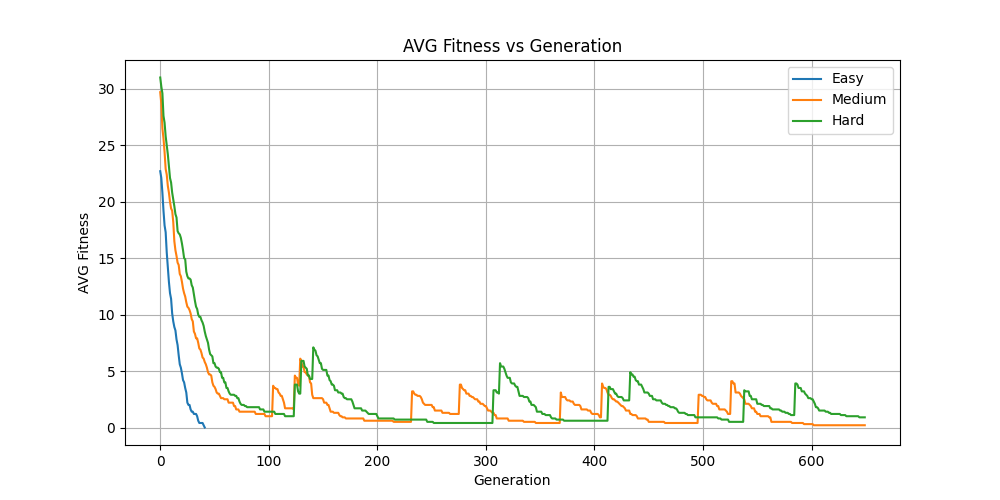
\includegraphics[width=\textwidth]{figures/plot.png}
	\caption{Average fitness value evaluated over 10 different Sudoku puzzles}
	\label{fig:avg_fitness}
\end{figure}
\end{document}
